%%%%%%%%%%%%%%%%%%%%%%%%%%%%%%%%%%%%%%%%%%%%%%%%
% Template productivity report
% 
% Alberto Sanchez asanchezrodelgo@ifc.org May 2016
%%%%%%%%%%%%%%%%%%%%%%%%%%%%%%%%%%%%%%%%%%%%%%%%
\documentclass{article}\usepackage[]{graphicx}\usepackage[]{color}
%% maxwidth is the original width if it is less than linewidth
%% otherwise use linewidth (to make sure the graphics do not exceed the margin)
\makeatletter
\def\maxwidth{ %
  \ifdim\Gin@nat@width>\linewidth
    \linewidth
  \else
    \Gin@nat@width
  \fi
}
\makeatother

\definecolor{fgcolor}{rgb}{0.345, 0.345, 0.345}
\newcommand{\hlnum}[1]{\textcolor[rgb]{0.686,0.059,0.569}{#1}}%
\newcommand{\hlstr}[1]{\textcolor[rgb]{0.192,0.494,0.8}{#1}}%
\newcommand{\hlcom}[1]{\textcolor[rgb]{0.678,0.584,0.686}{\textit{#1}}}%
\newcommand{\hlopt}[1]{\textcolor[rgb]{0,0,0}{#1}}%
\newcommand{\hlstd}[1]{\textcolor[rgb]{0.345,0.345,0.345}{#1}}%
\newcommand{\hlkwa}[1]{\textcolor[rgb]{0.161,0.373,0.58}{\textbf{#1}}}%
\newcommand{\hlkwb}[1]{\textcolor[rgb]{0.69,0.353,0.396}{#1}}%
\newcommand{\hlkwc}[1]{\textcolor[rgb]{0.333,0.667,0.333}{#1}}%
\newcommand{\hlkwd}[1]{\textcolor[rgb]{0.737,0.353,0.396}{\textbf{#1}}}%

\usepackage{framed}
\makeatletter
\newenvironment{kframe}{%
 \def\at@end@of@kframe{}%
 \ifinner\ifhmode%
  \def\at@end@of@kframe{\end{minipage}}%
  \begin{minipage}{\columnwidth}%
 \fi\fi%
 \def\FrameCommand##1{\hskip\@totalleftmargin \hskip-\fboxsep
 \colorbox{shadecolor}{##1}\hskip-\fboxsep
     % There is no \\@totalrightmargin, so:
     \hskip-\linewidth \hskip-\@totalleftmargin \hskip\columnwidth}%
 \MakeFramed {\advance\hsize-\width
   \@totalleftmargin\z@ \linewidth\hsize
   \@setminipage}}%
 {\par\unskip\endMakeFramed%
 \at@end@of@kframe}
\makeatother

\definecolor{shadecolor}{rgb}{.97, .97, .97}
\definecolor{messagecolor}{rgb}{0, 0, 0}
\definecolor{warningcolor}{rgb}{1, 0, 1}
\definecolor{errorcolor}{rgb}{1, 0, 0}
\newenvironment{knitrout}{}{} % an empty environment to be redefined in TeX

\usepackage{alltt}
%%%%%%%%%%%%%% package declaration %%%%%%%%%%%%%%%%%%%%%
\usepackage{fancyhdr}
\pagestyle{fancy}
\lhead{This is my name}
\rhead{this is page \thepage}
\cfoot{center of the footer!}
\usepackage[top=0.3in, bottom=0.1in, left=0.5in, right=0.6in]{geometry}
\usepackage{graphicx} % to load images
\usepackage[export]{adjustbox} % add alignment to includegraphics
\usepackage[font=small]{caption}
\usepackage{xcolor} % color text
\usepackage{tabularx} % to adjust table width, etc. 
\usepackage{titlesec} % format titles and headers
\usepackage{sectsty} % format sections & subsections
\usepackage{booktabs} % For \toprule, \midrule and \bottomrule
\usepackage{longtable} % add pages for long tables
\usepackage[colorlinks = true,
            linkcolor = blue,
            urlcolor  = blue,
            citecolor = blue,
            anchorcolor = blue]{hyperref} % to include hyperlinks in the doc
\sectionfont{\fontsize{24}{22}\selectfont\raggedright} % formats title newsletter (section) 
\subsectionfont{\fontsize{14}{12}\selectfont\raggedright} % formats title newsletter (section)
%%%%%%%%%%%%%%%%%%%%%%%%%%%%%%%%%%%%%%%%%%%%%%%%%%%%%%%%%%%%%%%%%%%%%%%%%%%%%%%%%%%
%
%%%%%%%%%%%%%%%%%%%%%%%%%%%%%%%%%%%%% BEGIN DOCUMENT %%%%%%%%%%%%%%%%%%%%%%%%%%%%%%
\IfFileExists{upquote.sty}{\usepackage{upquote}}{}
\begin{document}

%

%%%%%%%%%%%%%%%% PAGE 1 %%%%%%%%%%%%%%%%%%%
%World Bank logo and TCMN branding
\begin{figure}
  \vspace{-3ex} % move up this figure
  \hspace{-7ex} % move left this figure
  \includegraphics[width=5cm]{/Users/asanchez3/shinyTCMN/www/wb_logo_background.png}
\end{figure}
%\begin{figure}
 \begin{minipage}[t]{1.1\textwidth} % top section
      \vspace{-30ex}
      \hspace{10ex}
      \raggedleft{\section*{\color{white!20!black}Productivity Indicators Report}}
      %\raggedright{\includegraphics[width=5.5cm,right]{/Users/asanchez3/shinyTCMN/www/TC_snapshots_operations.png}}
  \end{minipage}
  
%\end{figure}
%
%%%% Macro Indicators
\begin{minipage}[t]{0.99\textwidth} % top section
  \vspace{-0.5cm}
      \subsection*{\color{white!40!black}Sector: \color{blue!40!black}Manufacturing}
      \subsection*{\color{white!40!black}Firm type: \color{blue!40!black}By size}
      \subsection*{\color{white!40!black}Indicator: \color{blue!40!black}Total factor productivity YKLM: Basic metals}
  \end{minipage} % end top section

\vspace*{1.5cm}
  \raggedright{\color{white!30!black} \textbf{\Large Summary Statistics}}
    \begin{minipage}[c]{0.99\textwidth}  
      \vspace*{0.2cm}
      
% latex table generated in R 3.2.2 by xtable 1.7-4 package
% Sun May  1 17:38:40 2016
{\footnotesize
\begin{tabular}{>{\raggedright}p{0.6in}>{\raggedleft}p{0.6in}>{\raggedleft}p{0.6in}>{\raggedleft}p{0.6in}>{\raggedleft}p{0.6in}>{\raggedleft}p{0.6in}>{\raggedleft}p{0.6in}>{\raggedleft}p{0.6in}>{\raggedleft}p{0.6in}>{\raggedleft}p{0.6in}l}
  & mean\_Large.firms & median\_Large.firms & sd\_Large.firms & mean\_Medium.firms & median\_Medium.firms & sd\_Medium.firms & mean\_Small.firms & median\_Small.firms & sd\_Small.firms &  \\ 
  \hline
Min & -1.02 & 0.35 & 0.34 & 0.90 & 0.42 & 0.45 & 1.04 & 0.26 & 0.36 &  \\ 
  Max & 1.64 & 0.72 & 0.95 & 1.40 & 0.61 & 0.61 & 1.33 & 0.50 & 0.60 &  \\ 
  Mean & 1.05 & 0.47 & 0.67 & 1.18 & 0.50 & 0.55 & 1.19 & 0.39 & 0.47 &  \\ 
  Median & 1.40 & 0.45 & 0.69 & 1.28 & 0.52 & 0.56 & 1.20 & 0.41 & 0.47 &  \\ 
  Stdev & 1.02 & 0.14 & 0.24 & 0.20 & 0.08 & 0.06 & 0.14 & 0.10 & 0.12 &  \\ 
  IQR & 0.24 & 0.11 & 0.34 & 0.24 & 0.11 & 0.07 & 0.22 & 0.12 & 0.20 &  \\ 
  \end{tabular}
}

      \vspace*{0.5cm}
    \end{minipage}
    
    \begin{minipage}[c]{0.99\textwidth}  


{\centering 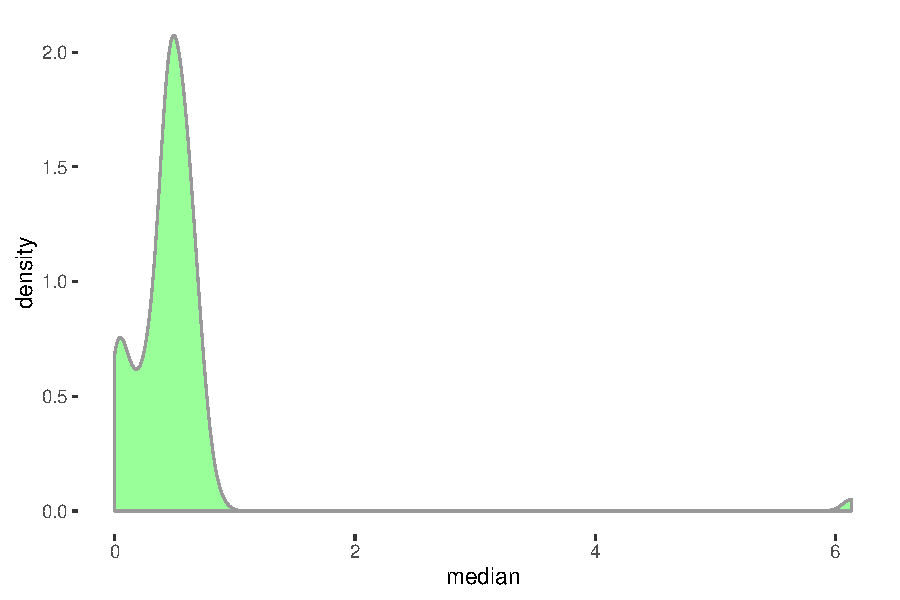
\includegraphics[width=\maxwidth]{figure/plot2-1} 

}



      \vspace*{0.5cm}
    \end{minipage}
%\end{minipage}

\newpage

  \raggedright{\color{white!30!black} \textbf{\Large Income Level Statistics}}
    \begin{minipage}[c]{0.99\textwidth}  
      \vspace*{0.4cm}
      
% latex table generated in R 3.2.2 by xtable 1.7-4 package
% Sun May  1 17:38:40 2016
{\footnotesize
\begin{tabular}{>{\raggedright}p{0.6in}>{\raggedleft}p{0.6in}>{\raggedleft}p{0.6in}>{\raggedleft}p{0.6in}>{\raggedleft}p{0.6in}>{\raggedleft}p{0.6in}>{\raggedleft}p{0.6in}>{\raggedleft}p{0.6in}>{\raggedleft}p{0.6in}>{\raggedleft}p{0.6in}l}
  & median\_Large.firms & sd\_Large.firms & iqr\_Large.firms & median\_Medium.firms & sd\_Medium.firms & iqr\_Medium.firms & median\_Small.firms & sd\_Small.firms & iqr\_Small.firms &  \\ 
  \hline
Lower middle income & 1.52 & 0.49 & 0.8 & 1.17 & 0.52 & 0.55 & --- & --- & --- &  \\ 
  Upper middle income & 1.3 & 0.35 & 0.34 & 1.28 & 0.42 & 0.56 & 1.3 & 0.45 & 0.6 &  \\ 
  NA & --- & --- & --- & --- & --- & --- & --- & --- & --- &  \\ 
  Low income & -1.02 & 0.37 & 0.68 & --- & --- & --- & --- & --- & --- &  \\ 
  \end{tabular}
}

      \vspace*{1cm}
    \end{minipage}
    
    \begin{minipage}[c]{0.99\textwidth}  
    


{\centering 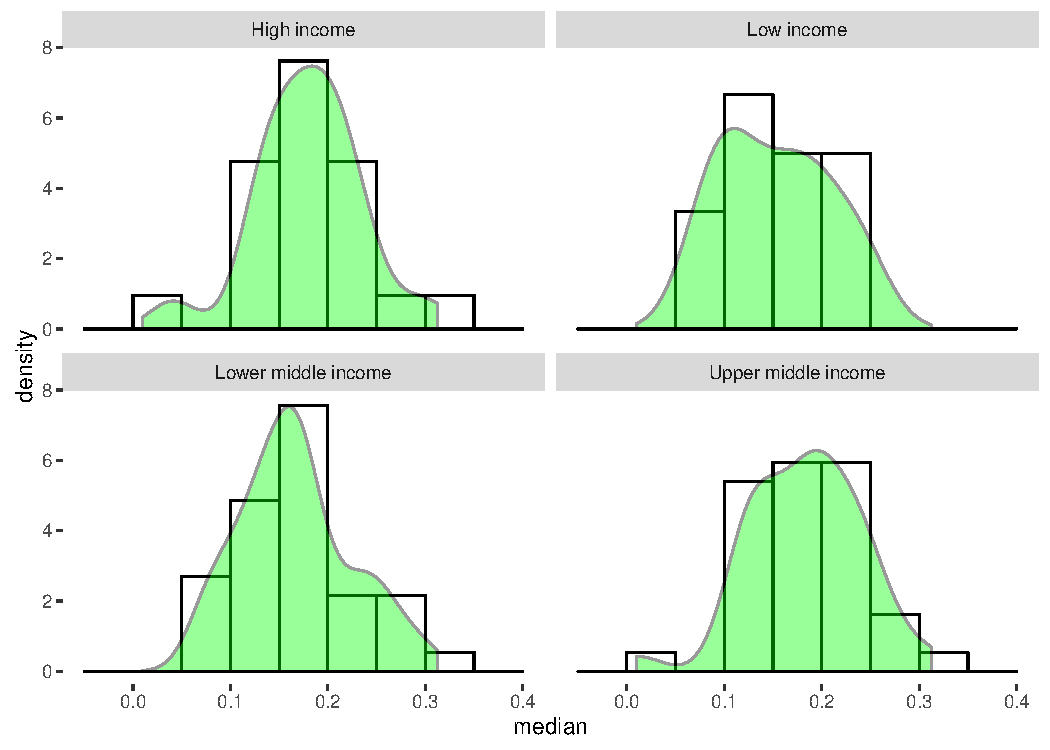
\includegraphics[width=\maxwidth]{figure/plot3-1} 

}



      \vspace*{0.5cm}
    \end{minipage}
%\end{minipage}

\newpage

  \raggedright{\color{white!30!black} \textbf{\Large Region Level Statistics}}
    \begin{minipage}[c]{0.99\textwidth}  
      \vspace*{0.4cm}
      
% latex table generated in R 3.2.2 by xtable 1.7-4 package
% Sun May  1 17:38:41 2016
{\footnotesize
\begin{tabular}{>{\raggedright}p{0.6in}>{\raggedleft}p{0.6in}>{\raggedleft}p{0.6in}>{\raggedleft}p{0.6in}>{\raggedleft}p{0.6in}>{\raggedleft}p{0.6in}>{\raggedleft}p{0.6in}>{\raggedleft}p{0.6in}>{\raggedleft}p{0.6in}>{\raggedleft}p{0.6in}l}
  & median\_Large.firms & sd\_Large.firms & iqr\_Large.firms & median\_Medium.firms & sd\_Medium.firms & iqr\_Medium.firms & median\_Small.firms & sd\_Small.firms & iqr\_Small.firms &  \\ 
  \hline
East Asia and Pacific & 1.43 & 0.38 & 0.52 & 1.16 & 0.52 & 0.51 & --- & --- & --- &  \\ 
  Middle East and North Africa & 1.64 & 0.72 & 0.91 & 0.9 & 0.52 & 0.61 & 1.04 & 0.26 & 0.38 &  \\ 
  South Asia & 1.32 & 0.49 & 0.68 & --- & --- & --- & --- & --- & --- &  \\ 
  \end{tabular}
}

      \vspace*{1cm}
    \end{minipage}
    
    \begin{minipage}[c]{0.99\textwidth}  
    


{\centering 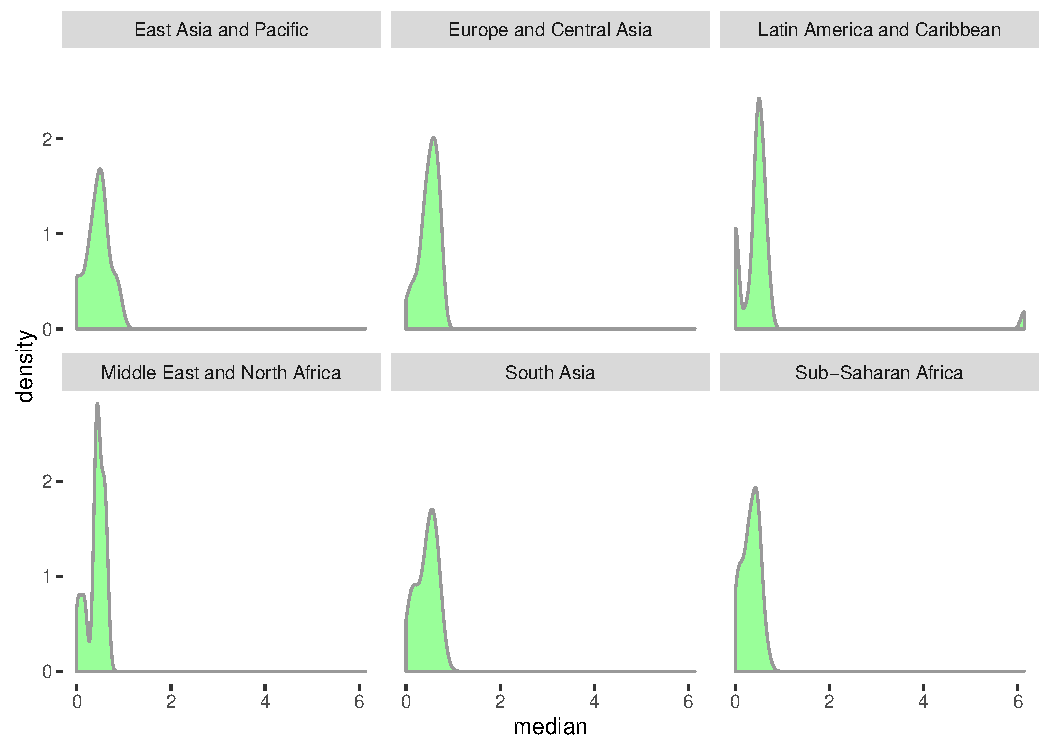
\includegraphics[width=\maxwidth]{figure/plot4-1} 

}



      \vspace*{0.5cm}
    \end{minipage}
%\end{minipage}

%%%%%%%%%%%%%%%% END OF DOCUMENT %%%%%%%%%%%%%%%%%%%
\end{document}
